\documentclass[a4paper,12pt]{article}

%%% Работа с русским языком
\usepackage{cmap}					% поиск в PDF
\usepackage{mathtext} 				% русские буквы в формулах
\usepackage[T2A]{fontenc}			% кодировка
\usepackage[utf8]{inputenc}			% кодировка исходного текста
\usepackage[english,russian]{babel}	% локализация и переносы
\usepackage{comment}


%%% Дополнительная работа с математикой
\usepackage{amsfonts,amssymb,amsthm,mathtools} % AMS
\usepackage{amsmath}
\usepackage{icomma} % "Умная" запятая: $0,2$ --- число, $0, 2$ --- перечисление

%% Номера формул
%\mathtoolsset{showonlyrefs=true} % Показывать номера только у тех формул, на которые есть \eqref{} в тексте.

%% Шрифты
\usepackage{euscript}	 % Шрифт Евклид
\usepackage{mathrsfs} % Красивый матшрифт

\usepackage{extsizes} % Возможность сделать 14-й шрифт
\usepackage{geometry} % Простой способ задавать поля
\geometry{top=25mm}
\geometry{bottom=35mm}
\geometry{left=15mm}
\geometry{right=15mm}

\usepackage{chngcntr}
\usepackage{hyperref}

\usepackage{setspace} % Интерлиньяж
%\onehalfspacing % Интерлиньяж 1.5
%\doublespacing % Интерлиньяж 2
%\singlespacing % Интерлиньяж 1

\usepackage{lastpage} % Узнать, сколько всего страниц в документе.
\usepackage{soulutf8} % Модификаторы начертания

\counterwithin*{equation}{section}
\counterwithin*{equation}{subsection}



%% Свои команды
\DeclareMathOperator{\sgn}{\mathop{sgn}}

%% Перенос знаков в формулах (по Львовскому)
\newcommand*{\hm}[1]{#1\nobreak\discretionary{}
{\hbox{$\mathsurround=0pt #1$}}{}}

%%% Работа с картинками
\usepackage{graphicx}  % Для вставки рисунков
\graphicspath{{images/}{images2/}}  % папки с картинками
\setlength\fboxsep{3pt} % Отступ рамки \fbox{} от рисунка
\setlength\fboxrule{1pt} % Толщина линий рамки \fbox{}
\usepackage{wrapfig} % Обтекание рисунков и таблиц текстом

%%% Работа с таблицами
\usepackage{array,tabularx,tabulary,booktabs} % Дополнительная работа с таблицами
\usepackage{longtable}  % Длинные таблицы
\usepackage{multirow} % Слияние строк в таблице
\usepackage{graphicx}
\usepackage{fancyhdr}
\usepackage{hyperref}
\usepackage{booktabs}

\newcommand{\lt}{\left}
\newcommand{\rt}{\right}
\newcommand{\al}{\alpha}
\newcommand{\p}{\partial}
\newcommand{\D}{\Delta}
\newcommand{\fr}{\frac}
\newcommand{\dfr}{\dfrac}
\newcommand{\mbf}{\mathbf}
\newcommand{\ol}{\overline}
\newcommand{\bb}{\mathbb}
\newcommand{\om}{\Omega}
\newcommand{\Rw}{\Rightarrow}
\newcommand{\ve}{\varepsilon}
\newcommand{\vp}{\varphi}


\pagestyle{fancy}
\fancyhf{}
\pagestyle{plain} % нумерация вкл.

\rhead{\today}
\lhead{Соколов Игорь, группа 573}

%%% Заголовок
\author{Соколов Игорь, группа 573}
\title{ДЗ по Теории Вероятностей к семинару №7.}
\date{\today}

\begin{document} % конец преамбулы, начало документа

\maketitle

\section{}

Найти функцию и плотность распределения суммы двух независимых случайных величин, которые распределены равномерно на отрезке [0, 1].

\vspace{\baselineskip}

\textbf{Решение:}

$\eta = \xi_1 + \xi_2$

\begin{equation}
F_{\eta}(u) = \bb P(\xi_1 +\xi_2 < u) = \iint\limits_{x_1 + x_2}f_{\xi_1,\xi_2}(x_1,x_2) = \int\limits_{-\infty}^{u}dy_2\int\limits_{-\infty}^{+\infty} f_{\xi_1, \xi_2}(y_1,y_2 - y_1)dy_1
\end{equation}

\begin{equation}
f_{\xi_1, \xi_2}(u) = \int\limits_{-\infty}^{+\infty} f_{\xi_1, \xi_2}(y, u -y)dy
\end{equation}

Получили формулу свертки.

Если $\xi_1$ и $\xi_2$ независимы, то справедливо
\begin{equation}
f_{\xi_1, \xi_2}(x) = \int\limits_{-\infty}^{+\infty} f_{\xi_1}(y) f_{\xi_2}(x-y)dy 
=
\begin{cases}
0,& x \notin[0;2]\\
x,& x \in[0;1]\\
2 - x,& x\in [1;2]
\end{cases}
\end{equation}

График $f_{\eta}(x)$

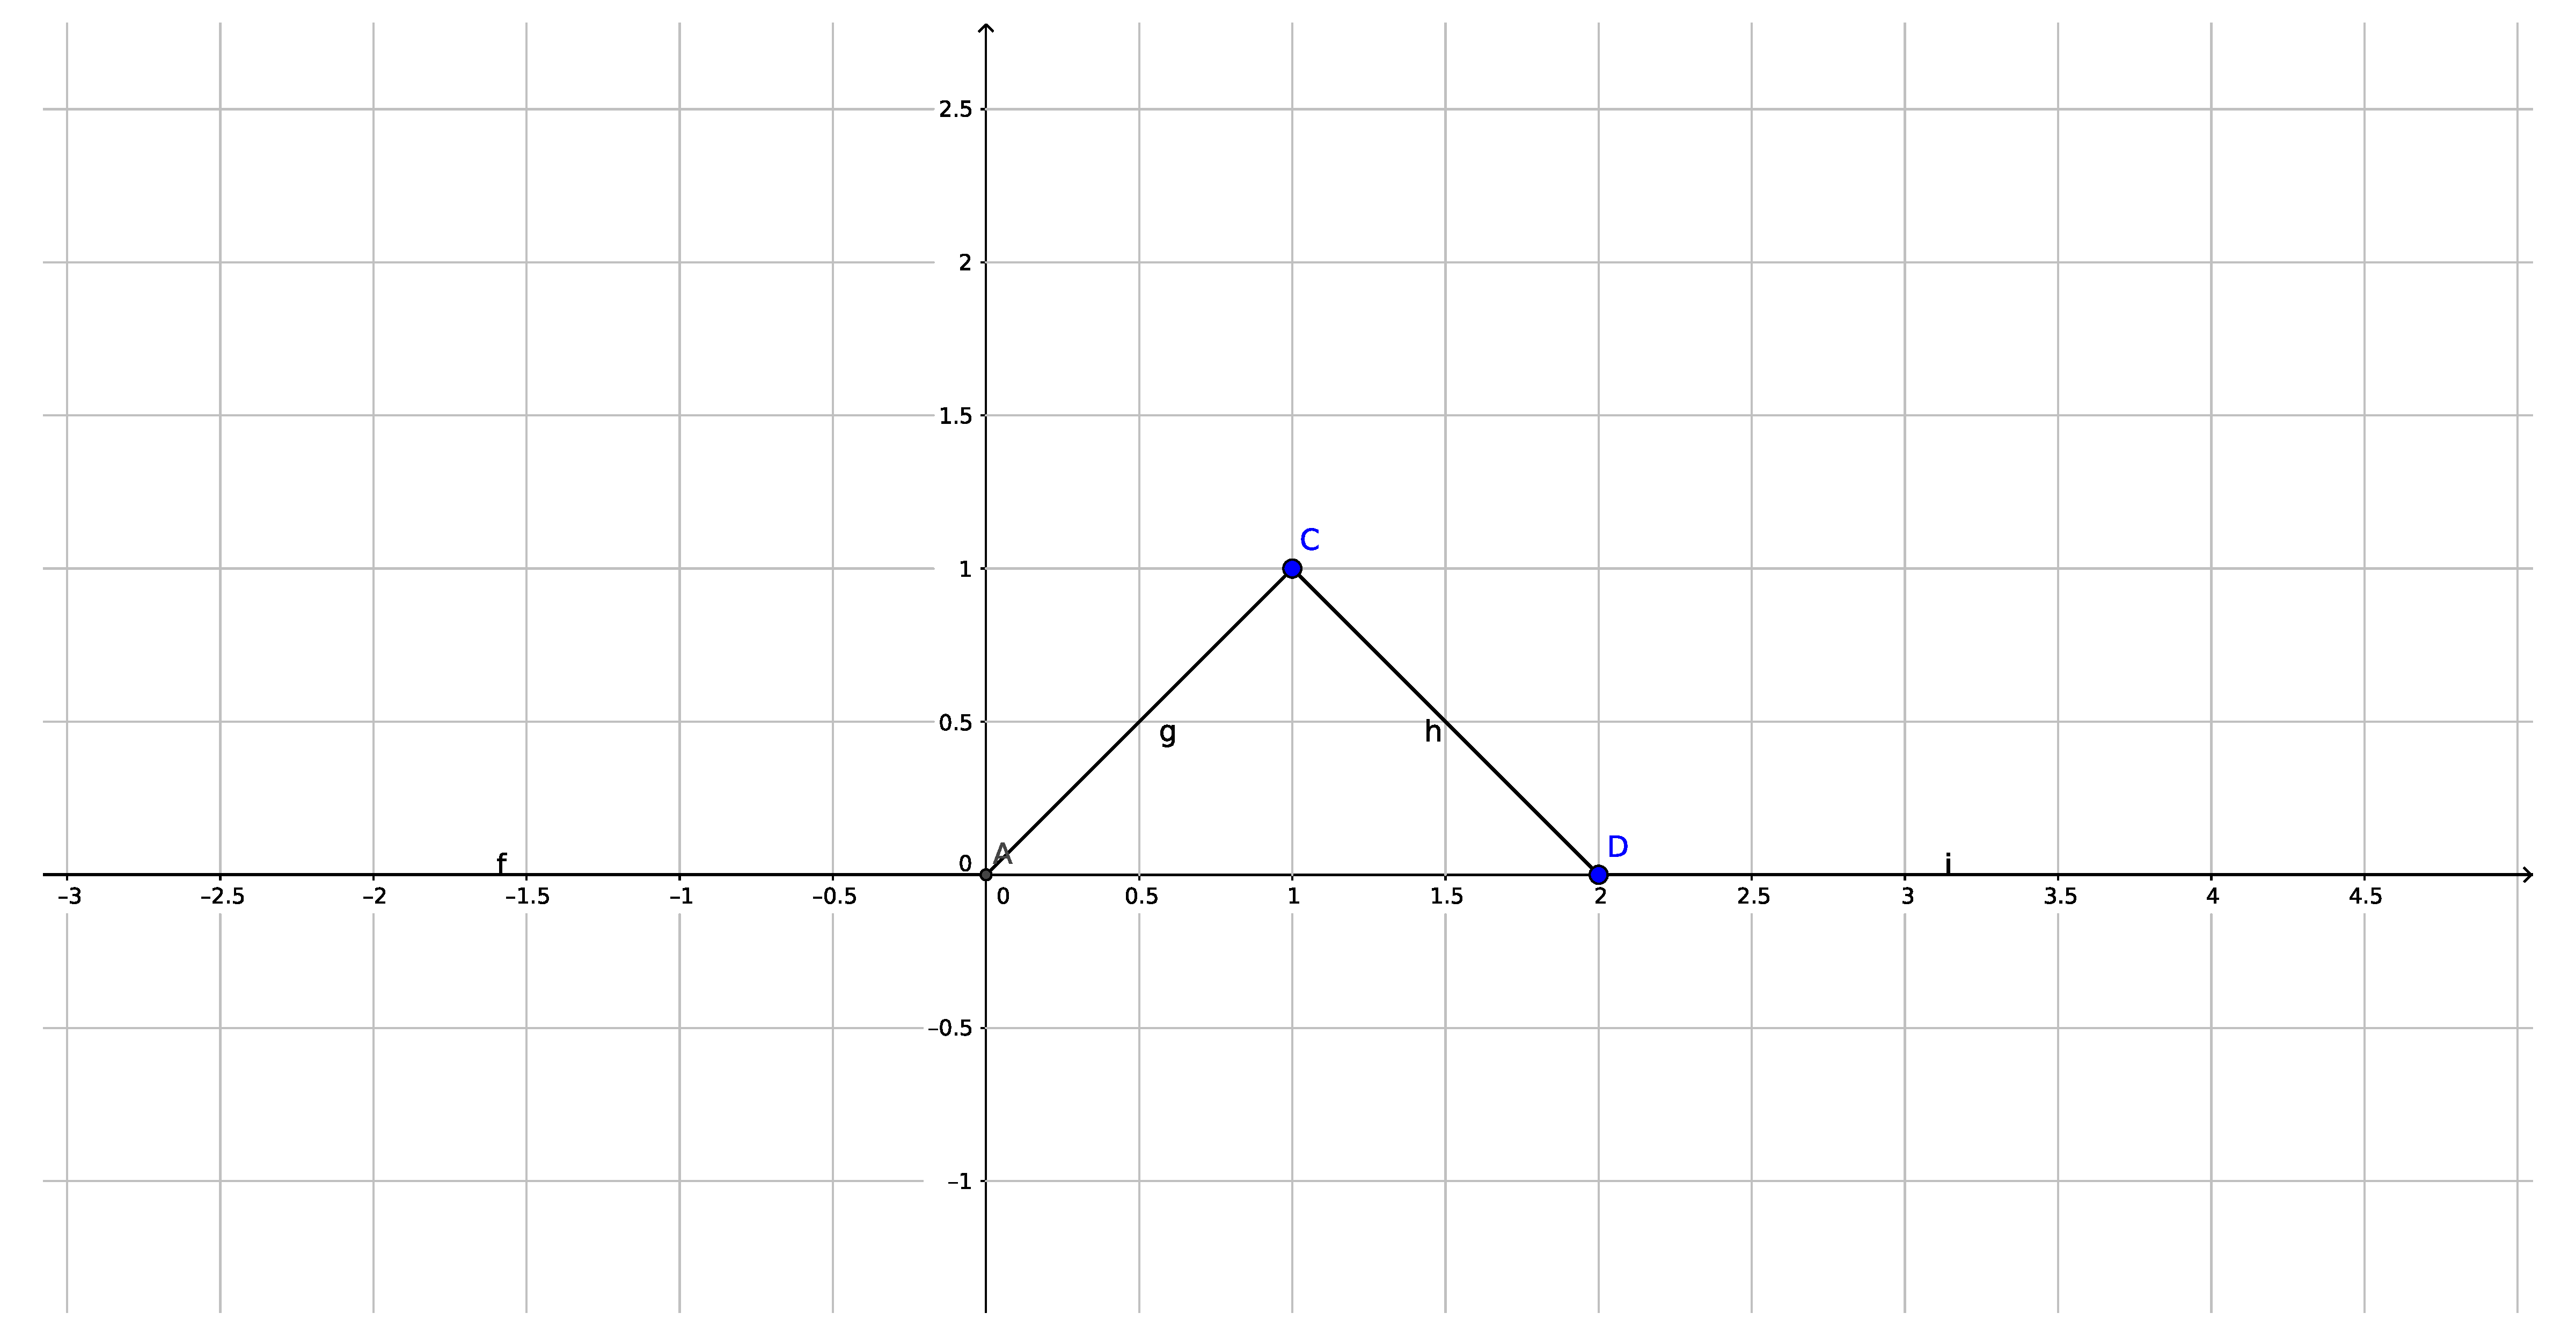
\includegraphics[width=\textwidth]{image1.pdf}

По опр 
\begin{equation}
F_{\eta}(x) = \int\limits_{-\infty}^{x}f_{\eta}(y)dy
\end{equation}

Найдем функцию распределения геометрически, посчитав площадь под графиком функции плотности.

Рассмотрим различные случаи:



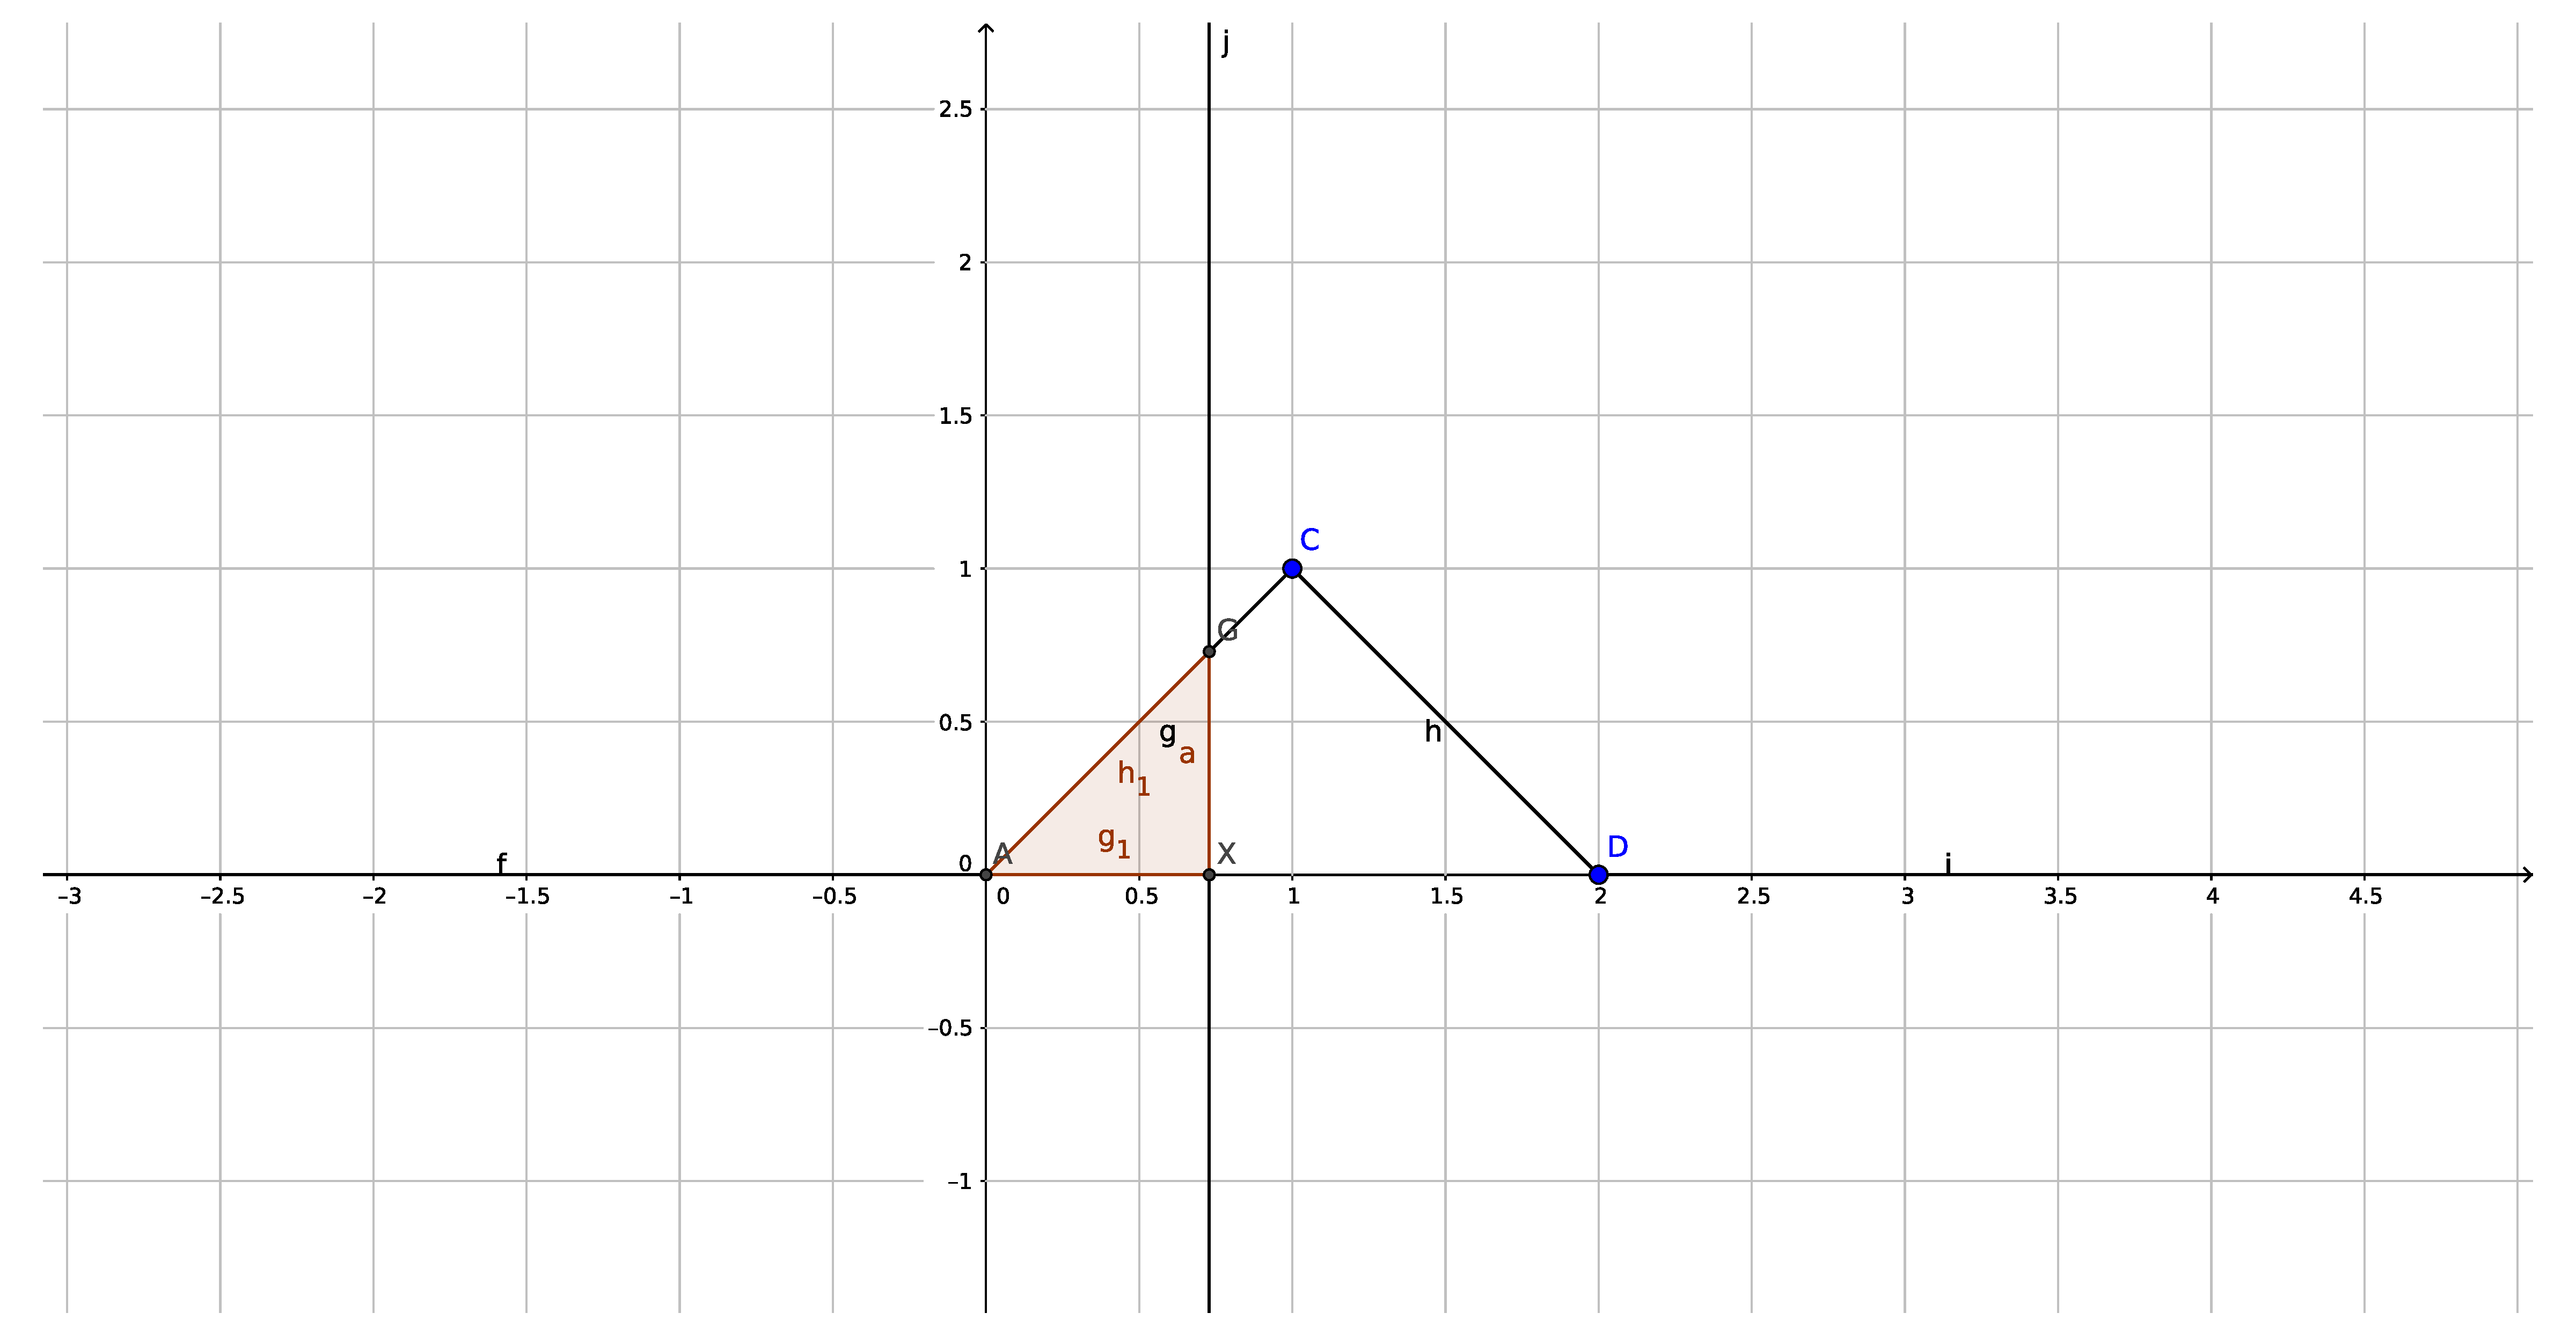
\includegraphics[width=\textwidth]{image2.pdf}

$x \in [0;1]$

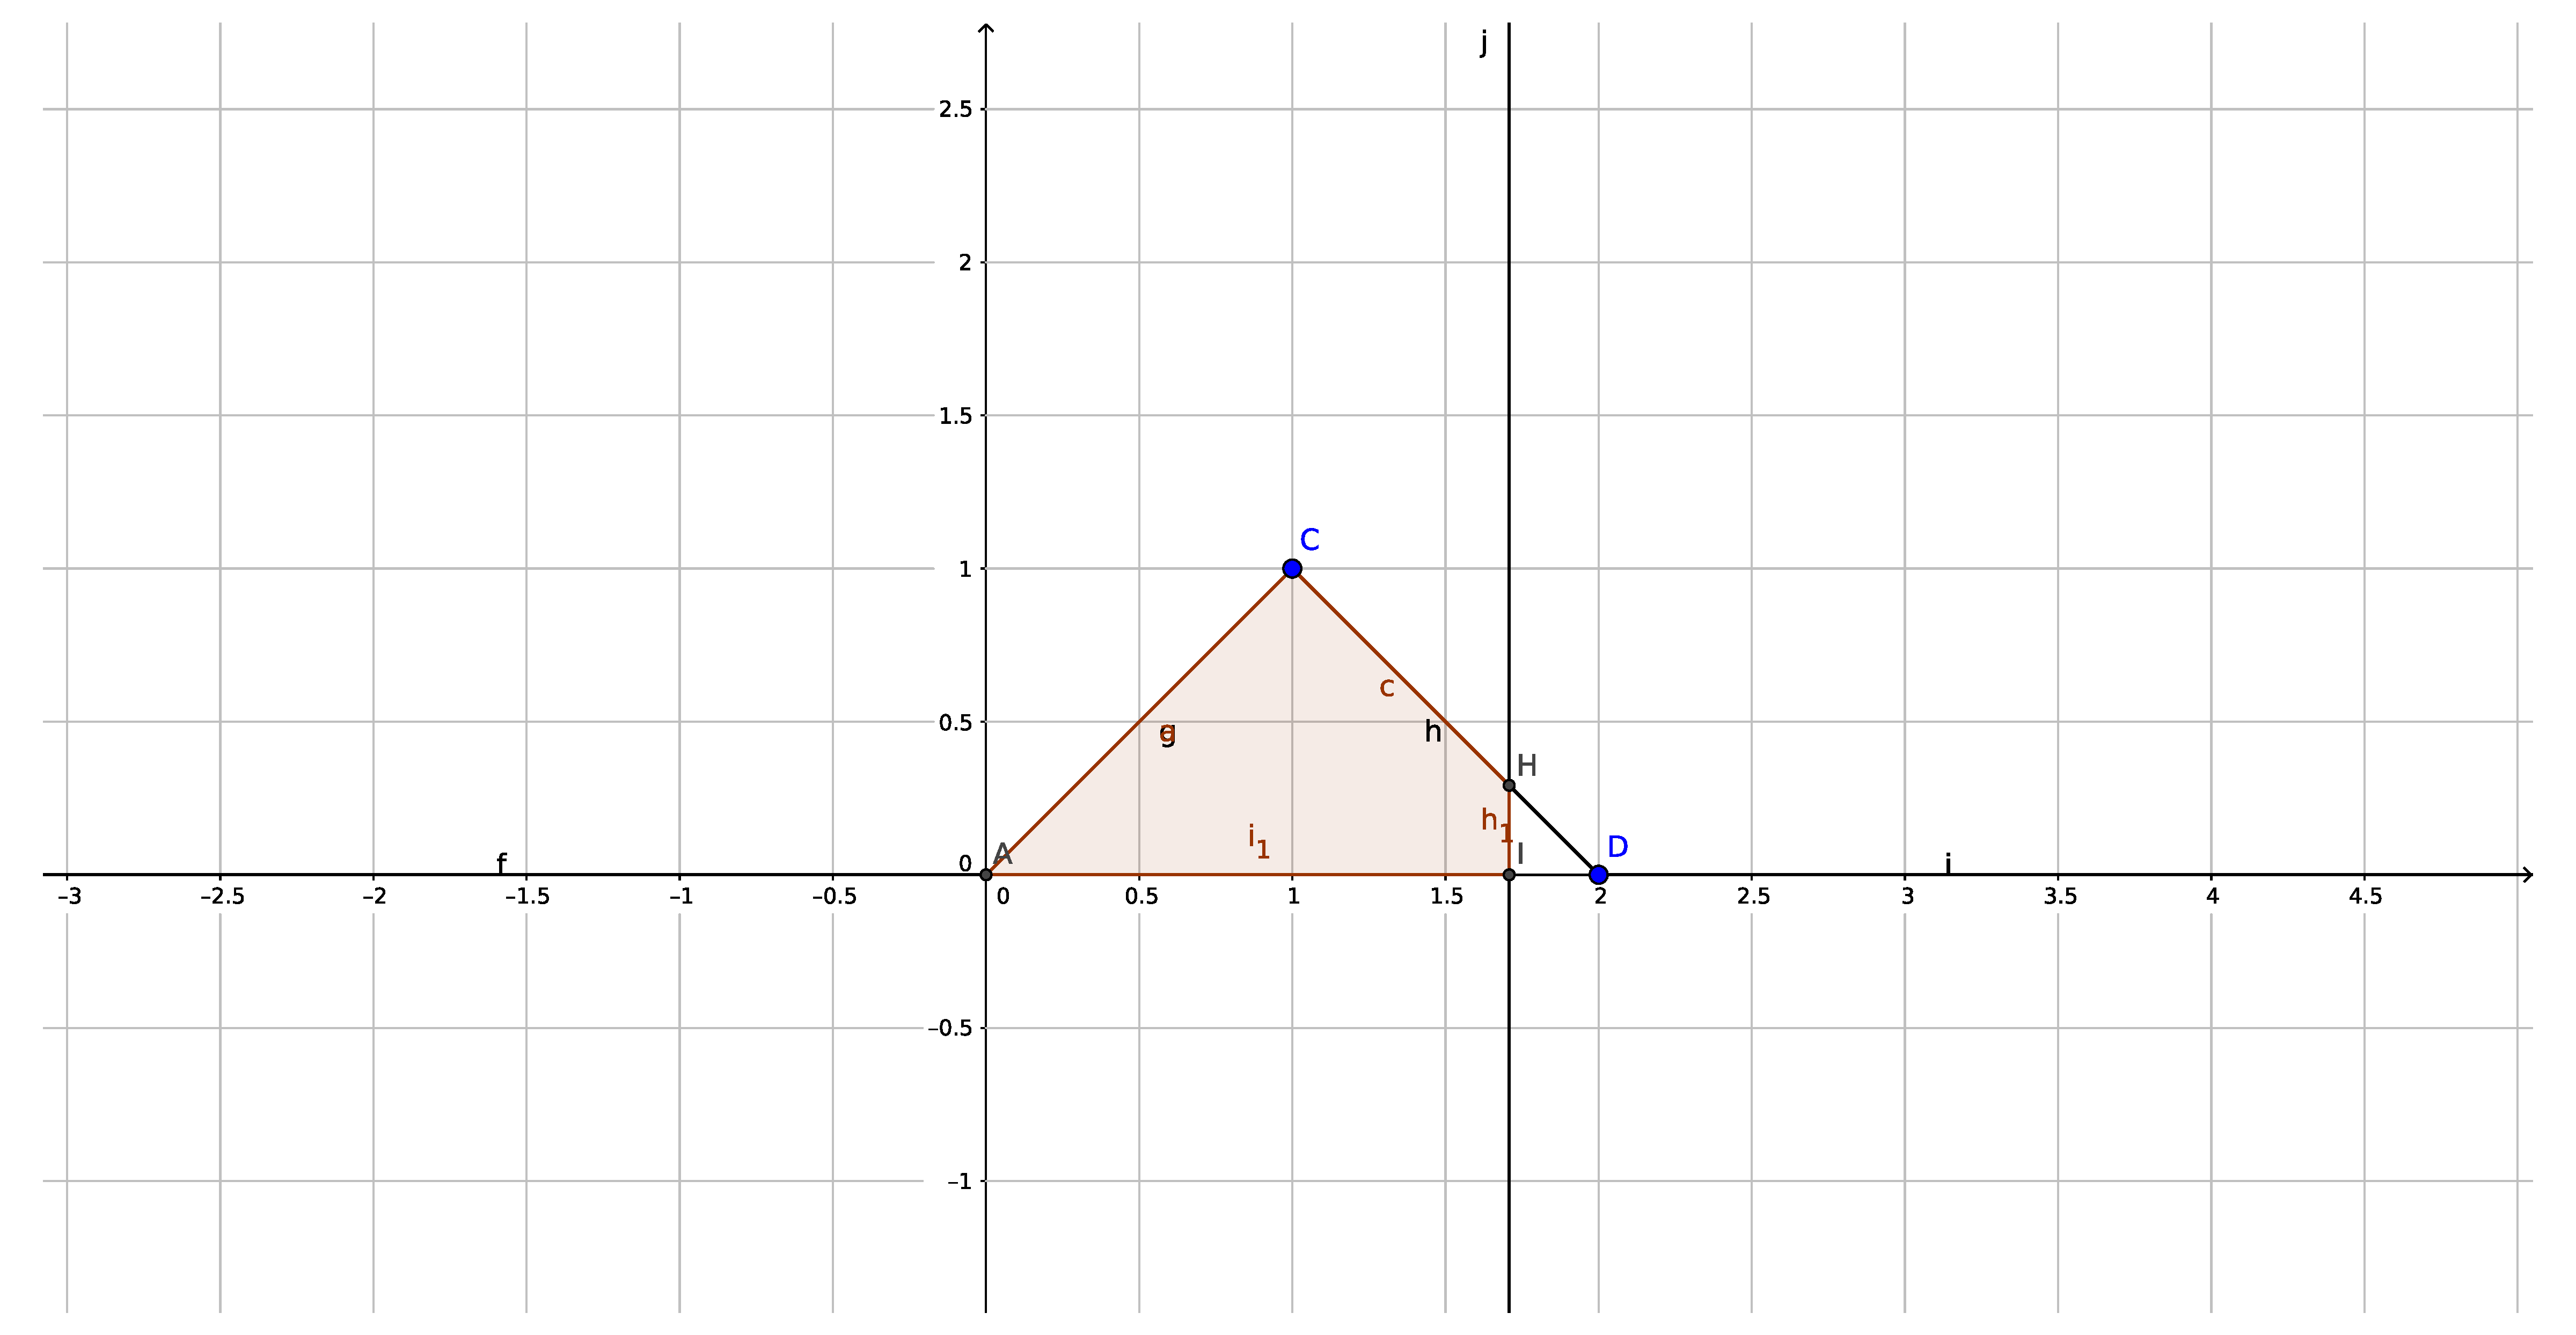
\includegraphics[width=\textwidth]{image3.pdf}

$x \in [1;2]$

Итого получаем:

\begin{equation}
F_{\eta}(x) = 
\begin{cases}
0,& x \notin[0;2]\\
\dfr{x^2}{2},& x \in[0;1]\\
1 - \dfr{(2 - x)^2}{2},& x\in [1;2]
\end{cases}
\end{equation}

\textbf{Ответ:}

$
f_{\xi_1 + \xi_2}(x)
=
\begin{cases}
	0,& x \notin[0;2]\\
	x,& x \in[0;1]\\
	2 - x,& x\in [1;2]
\end{cases}$

$F_{\xi_1 + \xi_2}(x) = 
\begin{cases}
0,& x \notin[0;2]\\
\dfr{x^2}{2},& x \in[0;1]\\
1 - \dfr{(2 - x)^2}{2},& x\in [1;2]
\end{cases}$


\end{document} % конец документа

